%%%%%%%%%%%%
%
% $Autor: Wings $
% $Datum: 2019-03-05 08:03:15Z $
% $Pfad: TemplateSensor $
% $Version: 4250 $
% !TeX spellcheck = en_GB/de_DE
% !TeX encoding = utf8
% !TeX root = filename 
% !TeX TXS-program:bibliography = txs:///biber
%
%%%%%%%%%%%%

% Structure
\chapter{DC-DC-Abwärtswandler}

In elektronischen Systemen werden unterschiedliche Spannungsbereiche benötigt. 
Mikrocontroller, Sensoren und weitere elektronische Baugruppen arbeiten mit niedrigen Gleichspannungen wie 3,3\,V oder 5\,V, während andere Komponenten höhere Versorgungsspannungen benötigen. 
Spannungswandler ermöglichen die Anpassung vorhandener Versorgungsspannungen an die jeweiligen Verbraucher.

Für die Versorgung von Mikrocontrollern und Logikschaltungen wird ein DC-DC-Abwärtswandler eingesetzt. 
Dieser reduziert eine höhere Eingangsspannung auf eine stabile Ausgangsspannung. 
Im Projekt wird hierfür ein Buck-Converter-Modul auf Basis des LM2596 beziehungsweise MP2307 verwendet.

Der Arduino Uno kann laut Datenblatt über den VIN-Anschluss mit einer Eingangsspannung von 6\,V bis 20\,V betrieben werden. 
Für den direkten Betrieb der Logikschaltungen wird jedoch eine stabile Versorgungsspannung von 5\,V benötigt \cite{Arduino:Uno}. 
Der eingesetzte DC-DC-Abwärtswandler übernimmt daher die Spannungsanpassung zwischen Netzteil und Mikrocontroller.

Im Gegensatz zu linearen Spannungsreglern arbeitet ein Abwärtswandler im Schaltbetrieb. 
Dadurch entstehen geringere Verlustleistungen und eine reduzierte Wärmeentwicklung. 
Gleichzeitig werden hohe Wirkungsgrade erreicht \cite{Schlienz:2020}.

\section{Eingesetzter Spannungswandler}

Für diese Anwendung wird ein einstellbarer DC-DC-Abwärtswandler verwendet, der auf dem LM2596 beziehungsweise MP2307 basiert. 
Das Modul reduziert die Eingangsspannung des Netzteils auf eine stabile Ausgangsspannung zur Versorgung des Arduino Uno sowie weiterer elektronischer Baugruppen.

Der eingesetzte Wandler besitzt eine kompakte Bauform, eine hohe Effizienz und lässt sich über Schraubklemmen in die Spannungsversorgung des Projekts integrieren. 
Aufgrund der Strombelastbarkeit eignet sich das Modul für Mikrocontroller-Anwendungen und kleinere elektronische Verbraucher.

\begin{center}
	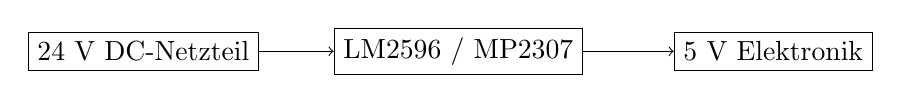
\begin{tikzpicture}[node distance=2cm, auto]
		\node (netzteil) [draw, rectangle] {24 V DC-Netzteil};
		\node (wandler) [right of=netzteil, draw, rectangle, node distance=4cm] {LM2596 / MP2307};
		\node (verbraucher) [right of=wandler, draw, rectangle, node distance=4cm] {5 V Elektronik};
		
		\draw[->] (netzteil) -- (wandler);
		\draw[->] (wandler) -- (verbraucher);
	\end{tikzpicture}
	\captionof{figure}{Blockschaltbild der Spannungsversorgung}
	\label{fig:dcdc_blockschaltbild}
\end{center}

\section{Spezifikation}

Das verwendete Modul besitzt folgende technische Eigenschaften \cite{MP2307:Datasheet}:

\begin{table}[H]
	\centering
	\caption{Technische Spezifikationen des LM2596-/MP2307-Abwärtswandlers}
	\label{tab:dcdc_specification}
	\begin{tabular}{ll}
		\hline
		\textbf{Eigenschaft} & \textbf{Wert} \\
		\hline
		Eingangsspannung & 4,75\,V bis 24\,V DC \\
		Ausgangsspannung & 0,93\,V bis 18\,V DC \\
		Ausgangsstrom & bis 2,5\,A dauerhaft \\
		Spitzenstrom & bis 4\,A \\
		Wirkungsgrad & bis 98\,\% \\
		Schaltfrequenz & ca. 150\,kHz \\
		Abmessungen & ca. 45\,mm $\times$ 32\,mm \\
		\hline
	\end{tabular}
\end{table}

Der Arduino Uno unterstützt laut Datenblatt Eingangsspannungen von 6\,V bis 20\,V am Anschluss \PYTHON{VIN} \cite{Arduino:Uno}. 
Die Versorgung über einen externen DC-DC-Wandler reduziert die Belastung des integrierten Spannungsreglers und verbessert die Energieeffizienz des Gesamtsystems.

\section{Funktionsprinzip}

Ein DC-DC-Abwärtswandler, auch Buck Converter genannt, reduziert eine Gleichspannung auf eine niedrigere Ausgangsspannung. 
Die Spannungsregelung erfolgt mithilfe eines schnell schaltenden MOSFETs. 
Durch das periodische Ein- und Ausschalten entsteht ein pulsierender Spannungsverlauf, der durch Induktivitäten und Kondensatoren geglättet wird \cite{Schlienz:2020}.

Der Betrieb des Abwärtswandlers erfolgt in mehreren Schritten. 
Zunächst schaltet der MOSFET die Eingangsspannung mit hoher Frequenz ein und aus. 
Während der Einschaltphase wird Energie in einer Induktivität gespeichert. 
In der Ausschaltphase gibt die Spule die gespeicherte Energie an den Ausgang ab. 
Kondensatoren glätten die entstehenden Spannungsschwankungen und stabilisieren die Ausgangsspannung.

Die Regelung der Ausgangsspannung erfolgt über das Tastverhältnis der Pulsweitenmodulation. 
Für den idealen Abwärtswandler gilt:

\[
\frac{U_a}{U_e} = v_T
\]

Die Ausgangsspannung \(U_a\) ergibt sich aus der Eingangsspannung \(U_e\) und dem Tastverhältnis \(v_T\) der PWM. 
Die Ausgangsspannung hängt somit direkt vom Tastverhältnis ab. 
Durch die hohe Schaltfrequenz kann eine kompakte und effiziente Spannungsregelung realisiert werden \cite{Schlienz:2020}.

\subsection{Wirkungsgrad}

Der Wirkungsgrad beschreibt das Verhältnis zwischen abgegebener und aufgenommener Leistung:

\[
\eta = \frac{P_{ab}}{P_{zu}} \cdot 100
\]

Dabei entspricht \(P_{ab}\) der abgegebenen Leistung und \(P_{zu}\) der aufgenommenen Leistung.

Durch den Schaltbetrieb erreicht der Abwärtswandler höhere Wirkungsgrade als lineare Spannungsregler. 
Beim verwendeten Modul sind Wirkungsgrade von bis zu 98\,\% möglich \cite{MP2307:Datasheet}.

\subsection{Verlustleistungen}

Trotz des hohen Wirkungsgrades entstehen innerhalb des Wandlers verschiedene Verlustleistungen. 
Dazu gehören Schaltverluste des MOSFETs, ohmsche Leitungsverluste sowie Verluste der Induktivität und der Kondensatoren.

Die Verlustleistung wird überwiegend in Wärme umgewandelt und führt zu einer Erwärmung der elektronischen Bauteile. 
Besonders bei höheren Lastströmen müssen diese Verluste berücksichtigt werden \cite{Schlienz:2020}.

\section{Schutzvorrichtungen}

Der eingesetzte DC-DC-Wandler verfügt über Schutzmechanismen zum Schutz der Elektronik.

\subsection{Überstromschutz}

Bei zu hohen Ausgangsströmen wird die Strombegrenzung aktiviert, um Schäden am Wandler und den angeschlossenen Komponenten zu vermeiden.

\subsection{Kurzschlussschutz}

Im Falle eines Kurzschlusses schützt sich der Wandler gegen zu hohe Ströme am Ausgang.

\subsection{Thermischer Schutz}

Bei zu hoher Temperatur reduziert der Wandler seine Leistung oder schaltet sich zum Schutz vor Überhitzung ab.

\section{Montage}

Der DC-DC-Abwärtswandler wird über Schraubklemmen mit der Spannungsversorgung und den elektronischen Verbrauchern verbunden.

Die Anschlüsse des Moduls sind:

\begin{itemize}
	\item \PYTHON{IN+}: positive Eingangsspannung
	\item \PYTHON{IN-}: Masse der Eingangsspannung
	\item \PYTHON{OUT+}: positive Ausgangsspannung
	\item \PYTHON{OUT-}: Masse der Ausgangsspannung
\end{itemize}

Die Eingangsspannung des Netzteils wird an \PYTHON{IN+} und \PYTHON{IN-} angeschlossen. 
Die reduzierte Ausgangsspannung liegt an \PYTHON{OUT+} und \PYTHON{OUT-} an. 
Vor dem Anschluss an den Arduino Uno und weitere elektronische Baugruppen wird die Ausgangsspannung mit einem Multimeter geprüft und über das Potentiometer des Wandlers auf 5\,V eingestellt.

Anschließend kann die Ausgangsspannung mit dem Arduino Uno sowie weiteren elektronischen Baugruppen verbunden werden. 
Dabei ist auf eine gemeinsame Masseverbindung der beteiligten Baugruppen zu achten.

\section{Weiterführende Literatur}

\begin{itemize}
	\item Schlienz, Ulrich: \textit{Schaltnetzteile und ihre Peripherie}. Springer Vieweg, 2020. \cite{Schlienz:2020}
	\item Erickson, Robert W. und Maksimovic, Dragan: \textit{Fundamentals of Power Electronics}. Springer, 2020.
	\item Arduino: \textit{Arduino Uno Rev3 Datasheet}. Technisches Datenblatt, 2025. \cite{Arduino:Uno}
	\item MP2307 / LM2596: \textit{DC-DC Converter Buck Module}. Technisches Datenblatt. \cite{MP2307:Datasheet}
\end{itemize}

% Schaltung ergänzen

%\section{Messung der Ausgangsspannung}

%\section{Überwachung der Spannungsversorgung}

%\subsection{Schaltung}

%\subsection{Code}